\section{S}
\subsection*{Material ID: mp-bfqdk}
\textbf{Constante Dieléctrica ($\epsilon_{total}$):} 4.31 \\[0.5em]
\begin{table}[h!]
\centering
\begin{tabular}{lcc}
\toprule
\textbf{Métrica} & \textbf{Lámina (Plate)} & \textbf{Cilindros (Rod)} \\
\midrule
Bandgaps ($a/\lambda$) & Ninguno & Ninguno \\
Resonancias & 36 & 36 \\
\bottomrule
\end{tabular}
\end{table}
\begin{figure}[H]
\centering
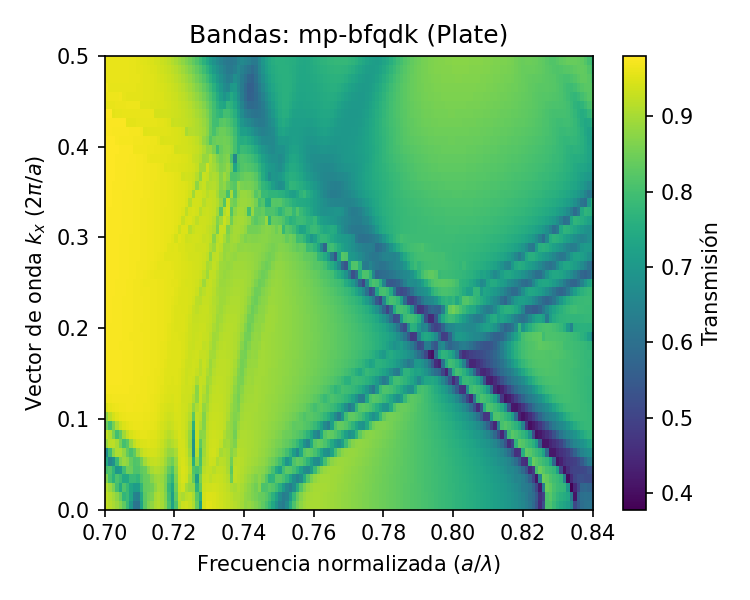
\includegraphics[width=0.48\textwidth]{figures/mp-bfqdk_plate.png}
\hfill
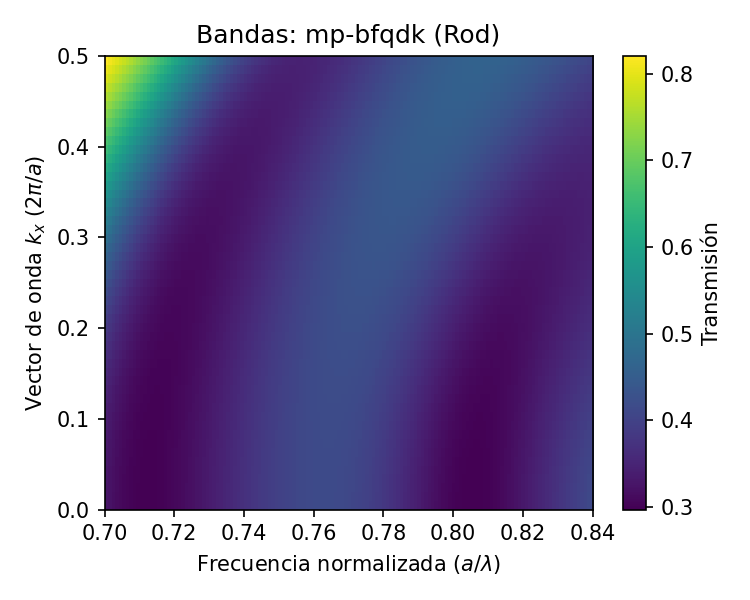
\includegraphics[width=0.48\textwidth]{figures/mp-bfqdk_rod.png}
\caption{Estructuras de bandas fotónicas para mp-bfqdk. Izquierda: Lámina. Derecha: Cilindros.}
\end{figure}
\vspace{1em}
\hrule
\vspace{1em}
\subsection*{Material ID: mp-bftmc}
\textbf{Constante Dieléctrica ($\epsilon_{total}$):} 3.09 \\[0.5em]
\begin{table}[h!]
\centering
\begin{tabular}{lcc}
\toprule
\textbf{Métrica} & \textbf{Lámina (Plate)} & \textbf{Cilindros (Rod)} \\
\midrule
Bandgaps ($a/\lambda$) & Ninguno & Ninguno \\
Resonancias & 36 & 36 \\
\bottomrule
\end{tabular}
\end{table}
\begin{figure}[H]
\centering
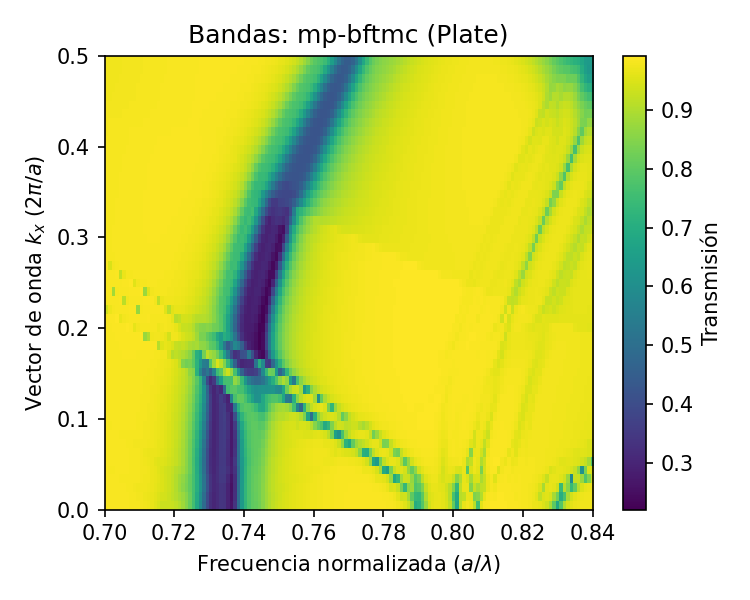
\includegraphics[width=0.48\textwidth]{figures/mp-bftmc_plate.png}
\hfill
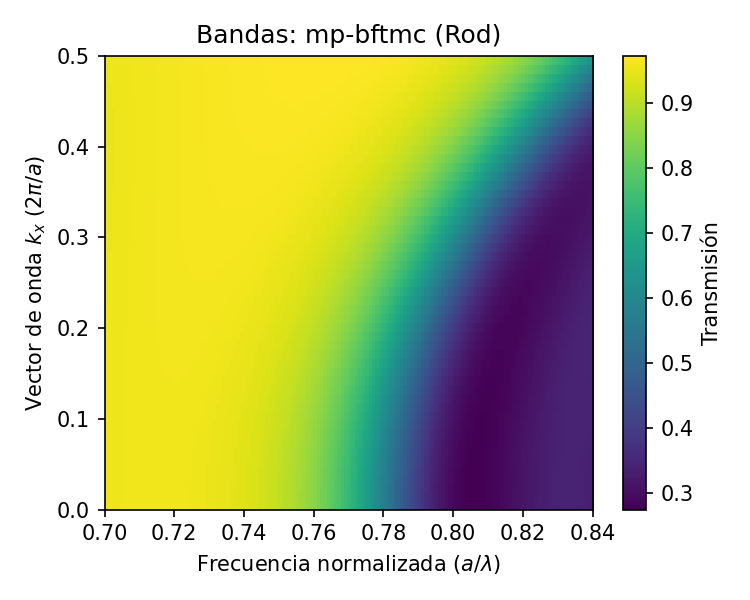
\includegraphics[width=0.48\textwidth]{figures/mp-bftmc_rod.png}
\caption{Estructuras de bandas fotónicas para mp-bftmc. Izquierda: Lámina. Derecha: Cilindros.}
\end{figure}
\vspace{1em}
\hrule
\vspace{1em}
\subsection*{Material ID: mp-bfyqr}
\textbf{Constante Dieléctrica ($\epsilon_{total}$):} 3.44 \\[0.5em]
\begin{table}[h!]
\centering
\begin{tabular}{lcc}
\toprule
\textbf{Métrica} & \textbf{Lámina (Plate)} & \textbf{Cilindros (Rod)} \\
\midrule
Bandgaps ($a/\lambda$) & Ninguno & Ninguno \\
Resonancias & 36 & 36 \\
\bottomrule
\end{tabular}
\end{table}
\begin{figure}[H]
\centering
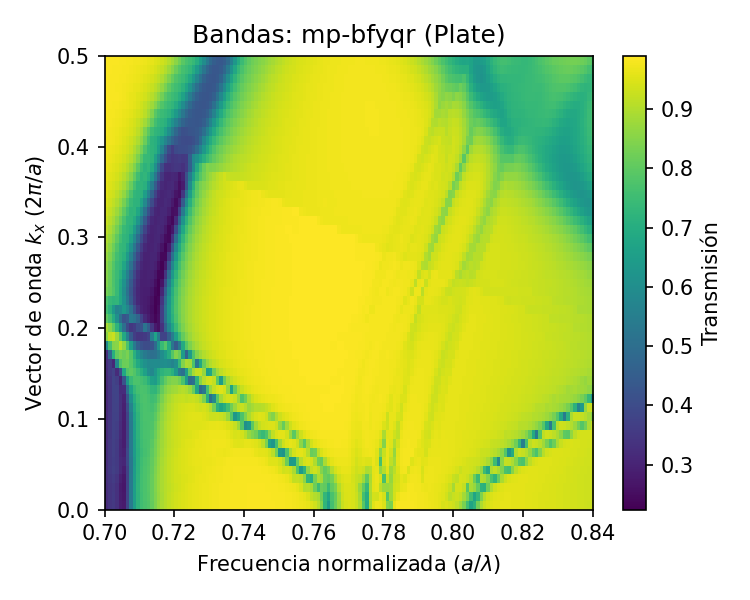
\includegraphics[width=0.48\textwidth]{figures/mp-bfyqr_plate.png}
\hfill
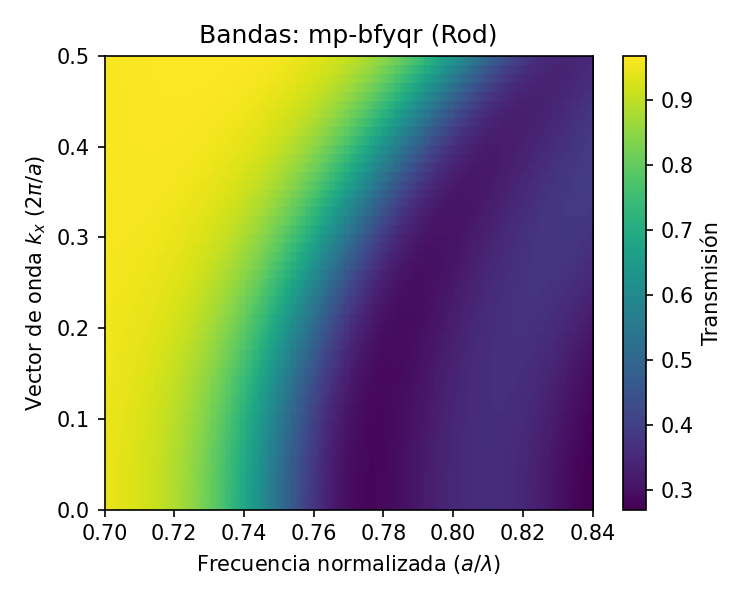
\includegraphics[width=0.48\textwidth]{figures/mp-bfyqr_rod.png}
\caption{Estructuras de bandas fotónicas para mp-bfyqr. Izquierda: Lámina. Derecha: Cilindros.}
\end{figure}
\vspace{1em}
\hrule
\vspace{1em}
\subsection*{Material ID: mp-cz}
\textbf{Constante Dieléctrica ($\epsilon_{total}$):} 2.95 \\[0.5em]
\begin{table}[h!]
\centering
\begin{tabular}{lcc}
\toprule
\textbf{Métrica} & \textbf{Lámina (Plate)} & \textbf{Cilindros (Rod)} \\
\midrule
Bandgaps ($a/\lambda$) & Ninguno & Ninguno \\
Resonancias & 36 & 36 \\
\bottomrule
\end{tabular}
\end{table}
\begin{figure}[H]
\centering
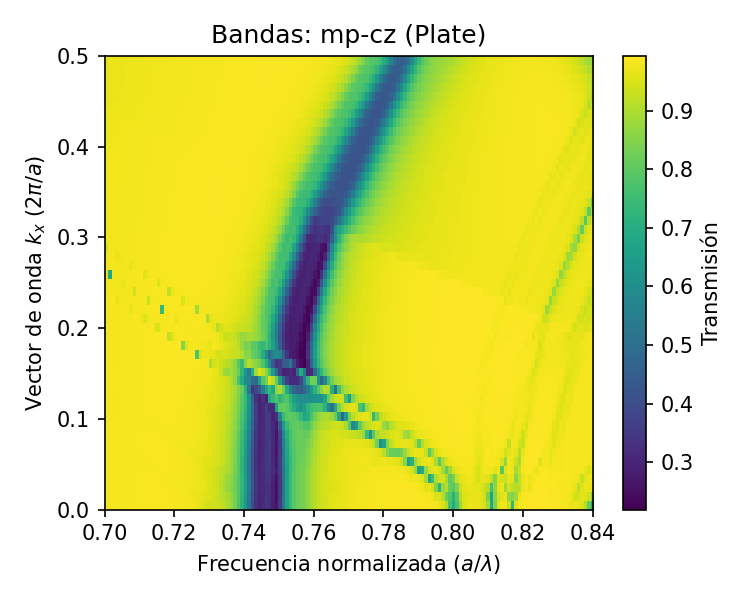
\includegraphics[width=0.48\textwidth]{figures/mp-cz_plate.png}
\hfill
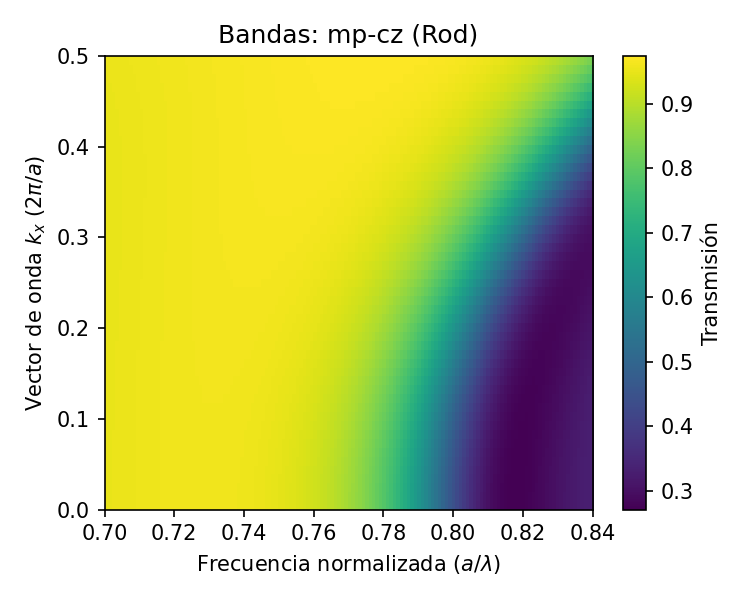
\includegraphics[width=0.48\textwidth]{figures/mp-cz_rod.png}
\caption{Estructuras de bandas fotónicas para mp-cz. Izquierda: Lámina. Derecha: Cilindros.}
\end{figure}
\vspace{1em}
\hrule
\vspace{1em}
\clearpage